\section{REINFORCE in action: Recurrent Attention Model (RAM)}
\begin{frame}{}
    \LARGE REINFORCE in Action: \textbf{Recurrent Attention Model (RAM)}
\end{frame}

\begin{frame}{REINFORCE in Action: Recurrent Attention Model (RAM)}
    \begin{itemize}
        \item \textbf{Objective:} Image classification
        \item The model takes a sequence of “glimpses,” selectively focusing on regions of the image to predict the class.
        \begin{itemize}
            \item Inspired by human perception and eye movements
            \item Saves computational resources $\Rightarrow$ improves scalability
            \item Can ignore clutter or irrelevant parts of the image
        \end{itemize}
        \item \textbf{State:} Glimpses observed so far
        \item \textbf{Action:} $(x, y)$ coordinates (center of the next glimpse) indicating where to look next in the image
        \item \textbf{Reward:} 1 at the final timestep if the image is correctly classified, 0 otherwise
    \end{itemize}
    \footnotetext{[Mnih et al., 2014]}
\end{frame}

\begin{frame}{REINFORCE in Action: Recurrent Attention Model (RAM)}
    \begin{figure}
        \centering
        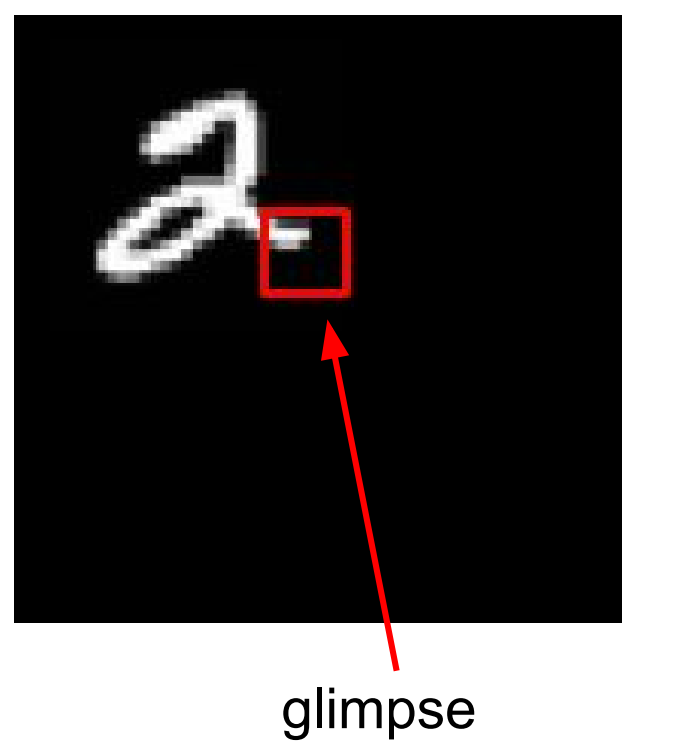
\includegraphics[width=0.9\textwidth,height=0.6\textheight,keepaspectratio]{images/policygrad+reinforce+actor/ram_1.png}
    \end{figure}
    \begin{itemize}
        \item Glimpsing is a non-differentiable operation.
        \item The policy for selecting glimpse locations is learned using REINFORCE.
        \item Given the sequence of glimpses observed so far, an RNN models the state and outputs the next action.
    \end{itemize}
    \footnotetext{[Mnih et al., 2014]}
\end{frame}

\begin{frame}{REINFORCE in Action: Recurrent Attention Model (RAM)}
    \begin{figure}
        \centering
        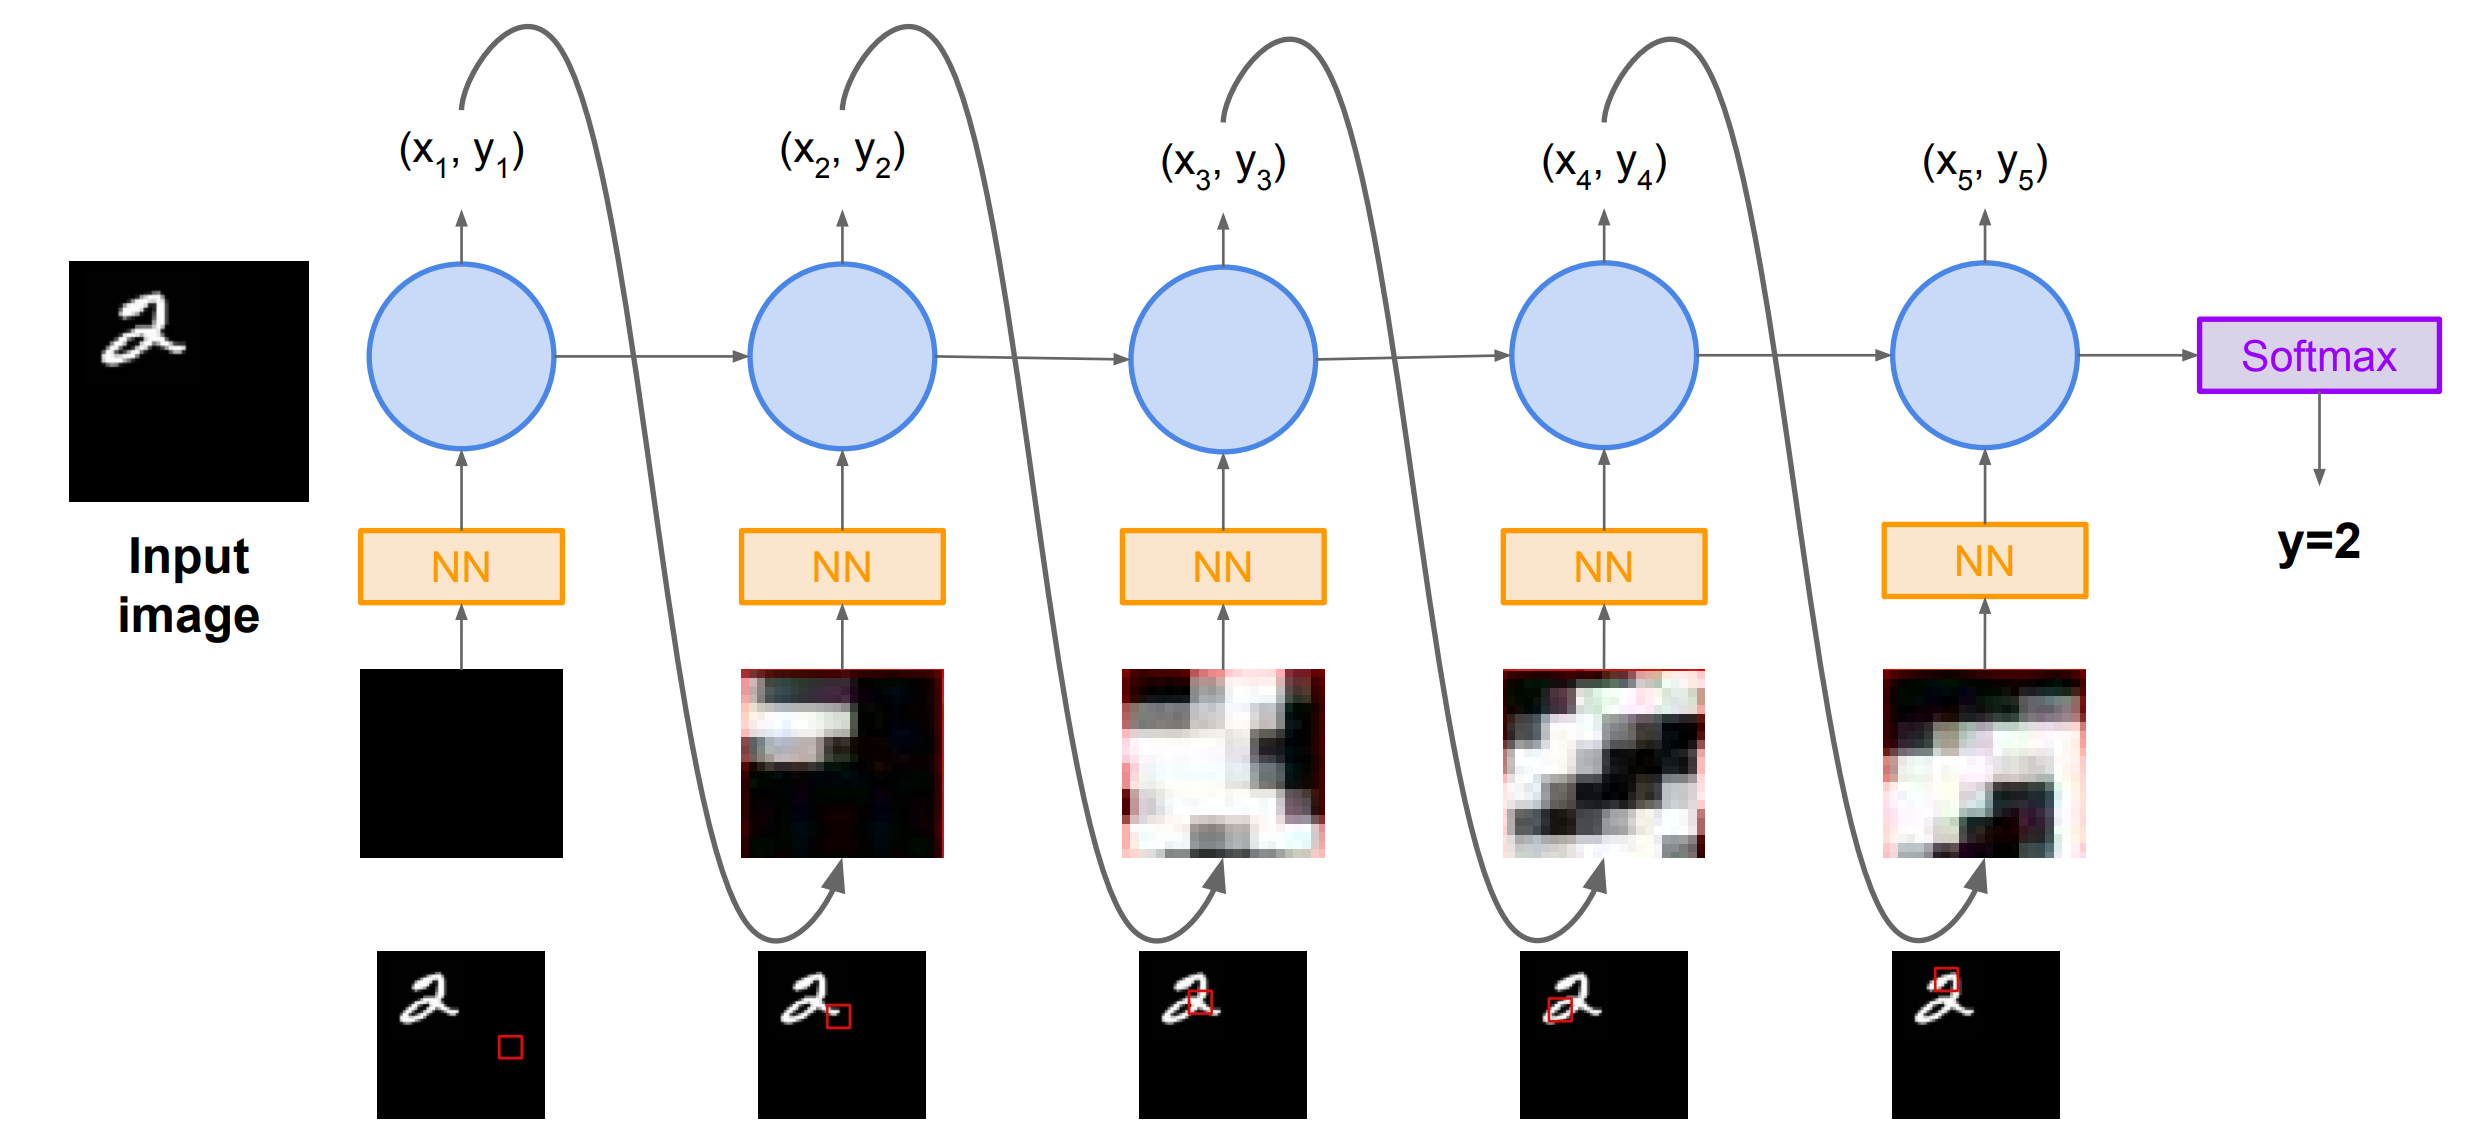
\includegraphics[width=1.0\textwidth,height=1.0\textheight,keepaspectratio]{images/policygrad+reinforce+actor/ram_2.png}
    \end{figure}
    \footnotetext{[Mnih et al., 2014]}
\end{frame}
